\chapter{Theoretische Grundlagen}
\label{chap:theo}

\section{Elektronen auf Helium}
Zu Beginn der siebziger Jahre des vorigen Jahrhunderts wurde von \name{M.~W.~Cole} \cite{Col69} und \name{V.~Shikin} \cite{Shi70} unabhängig voneinander die Existenz eines neuen Oberflächenzustands von Elektronen auf der Oberfläche von flüssigem Helium vorgeschlagen. Die Elektronen sind in der Ebene der Flüssigkeitsoberfläche frei beweglich und in der Richtung senkrecht dazu lokalisiert. Sie befinden sich dann in Zuständen, die den Zuständen des Elektrons im Wasserstoffatom sehr ähnlich sind.
Allerdings besitzen diese Zustände -- aufgrund der hier sehr viel schwächeren Bindung, die nur aus der Coulombkraft mit der Bildladung des Elektrons im Helium resultiert -- eine deutlich größere Bindungslänge und eine stark reduzierte Bindungsenergie.

Wenig später wurde ein Experiment  von \name{R.~Williams}, \name{R.~S.~Crandall} und \name{A.~H.~Willis} \cite{Wil71} durchgeführt, in dem die Lebensdauer eines solchen vorhergesagten Oberflächenzustandes unter verschiedenen äußeren Bedingungen untersucht wurde. \name{Williams} \ea{} haben eine Oberfläche flüssigen Heliums von der Gasseite her mit Elektronen beladen und konnten eine korrelierte Verringerung des elektrischen Feldes über der Heliumoberfläche messen. Durch kurzzeitiges Abschalten der positiven Spannung der die Elektronen anziehenden Halteelektrode im flüssigen Helium konnten sie so das Verschwinden der Elektronen des 2DES in den Gasraum hinein detektieren und somit die Lebensdauer dieses Zustandes ohne angelegte Haltespannung bestimmen.

Ein Experiment zur lateralen Beweglichkeit der Elektronen im 2DES -- also eine erste Transportmessung am 2DES -- wurde von \name{W.~T.~Sommer} und \name{D.~J.~Tanner} \cite{Som71} durchgeführt. Hierbei wurde die Beweglichkeit der Elektronen im 2DES über ihren Einfluss auf das elektrische Übersprechen zwischen zwei in einer Ebene unter dem flüssigen Helium liegenden Kondensatorplatten bestimmt.

\subsection{Das Potential der Elektronen im 2DES}
Im Jahre 1974 wurde dann von \name{C.~C.~Grimes} und \name{T.~R.~Brown} \cite{Gri74} ein direkter Beweis des Vorhandenseins der Oberflächenzustände der Elektronen vorgestellt. Die Energieniveaus der lokalisierten Elektronen wurden durch ihre  Absorption von Mikrowellen bei einer Frequenz in der Größenordnung von \unit[100]{GHz} nachgewiesen. Hier erhält man Absorptionslinien für die Übergänge $1\rightarrow2$ und $2\rightarrow3$, deren Energien charakteristisch für das schwach gebundene Elektronensystem auf flüssigem Helium sind.
Die Struktur des Potentials, in dem sich ein Elektron auf Bulk-Helium bewegt, konnte genauer überprüft werden. Dieses ist aus zwei Anteilen zusammengesetzt und entsteht alleine durch die Anwesenheit eines Elektrons selbst:

\begin{enumerate}
    \item In den oberen Halbraum hinein reicht ein schwaches, attraktives Coulomb"=Potential, das von der Bildladung erzeugt wird, die das Elektron im Dielektrikum Helium induziert.
    \item In der Nähe der Heliumoberfläche gibt es eine Barriere von etwa \unit[1]{eV}, die das Elektron überwinden muss, um in das flüssige Helium eindringen zu können. Diese Barriere ergibt sich aufgrund der Pauli-Abstoßung, die das Elektron durch die Anwesenheit der beiden $1s$-Elektronen der Heliumatome erfährt.

Da die Barriere mit ungefähr \unit[1]{eV} viel höher als die Tiefe des anziehenden Coulomb-Potentials von einigen meV ist, wird sie für Berechnungen der Wellenfunktion, Energie, etc.\ näherungsweise als unendlich hohe Barriere angenommen.
\end{enumerate}

\begin{figure}[h!tbp]
    \centerline{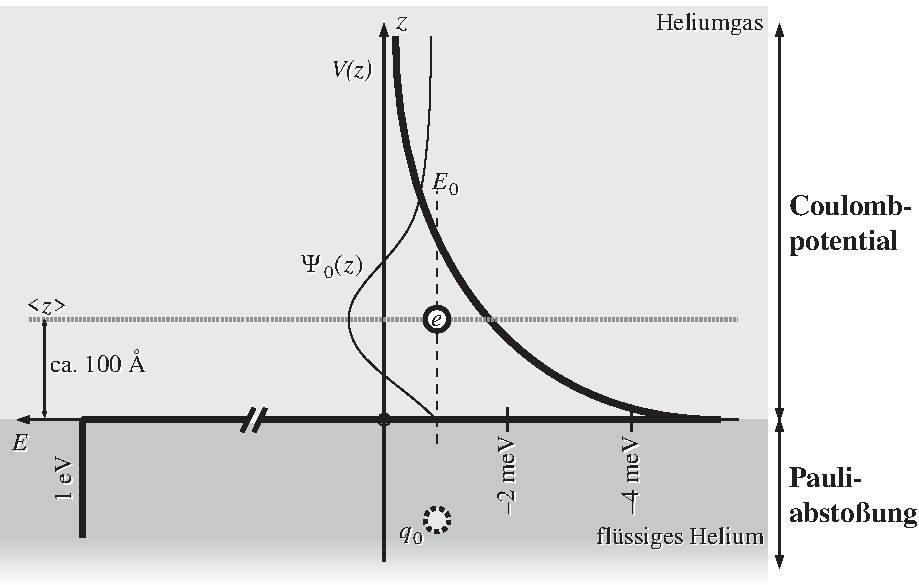
\includegraphics[width=\bigwidth]{theo_electrons_on_helium/SSE}}
    \caption[Das Potential, in dem sich ein Elektron auf flüssigem Helium bewegt.]{Das Potential, in dem sich ein Elektron auf flüssigem Helium bewegt. Am rechten Rand ist angezeigt, welcher Teil des Potentials für ein Elektron im jeweiligen Bereich dominiert.} 
    \label{fig:potential}
\end{figure}
Wenn man beide Anteile zu einem Gesamtpotential zusammenführt, das in Abbildung~\ref{fig:potential} schematisch dargestellt ist, erhält man folgenden Ausdruck:
    \begin{equation}
        \label{eqn:SSE_Potential}
        V(z)=\left\{\begin{array}{cl}
             V_0 & \;z\leq0\\
            -\frac{1}{4\pi\,\epsilon_0}\frac{q_0\,e^2}{z+\beta} & \;z>0\\
        \end{array}\right.
        \quad\textrm{mit}\quad
        \begin{array}{rl}
            V_0=&\unit[1]{eV}\\
            q_0=&\frac{\epsilon-1}{4(\epsilon+1)}\\
        \end{array}\quad.
    \end{equation}

Hierbei ist $q_0$ die Bildladung, deren Größe durch die \DK\ des Heliums bestimmt wird. Auf dünnen Heliumfilmen kommt noch die weit höhere Bildladung im Substrat hinzu. Der Offset $\beta$ ergibt sich nach \name{Grimes} \ea~\cite{Gri74} aus der physikalischen Tatsache, dass die Ebene, in der die Pauli-Abstoßung einsetzt durch die Überlappung der Wellenfunktionen der $1s$-Elektronen des Heliums mit der Wellenfunktion der 2D-Elektronen gegeben ist. Die Symmetrieebene der Bildladungen ist um ungefähr einen Atomradius dazu versetzt und verhindert für $\beta>0$ die Singularität des Potentials im $z$"=Koordinatenursprung. \name{Grimes} \ea\  bestimmten für $\beta$ etwa \unit[1]{\AA}, was näherungsweise mit dem Radius der Helium"=Atome übereinstimmt.

Die Lösung des Problems mit dem Potential aus Gleichung~\eqref{eqn:SSE_Potential} ist, bis auf die hier nicht vorhandene Kugelsymmetrie des Systems, identisch zur bekannten Lösung der Schrödingergleichung des Elektrons im Wasserstoffatom. Für den Bohrschen Radius ergibt sich hier aufgrund der im Vergleich zum Wasserstoffatom wesentlich schwächeren Bindung des Elektrons eine Länge von ca.\ \unit[114]{ \AA} (vgl. H-Atom \unit[0.5]{\AA}) und eine Grundzustandsenergie von $\unit[-0.65]{meV}$ (H-Atom $\unit[-13.6]{eV}$). Der Energieabstand zum ersten angeregten Zustand beträgt \unit[0.49]{meV}, was einer Temperatur von \unit[5.7]{K} entspricht; dies bedeutet, dass sich bei Temperaturen um \unit[1.5]{K} näherungsweise alle Elektronen im Grundzustand befinden und somit ein rein zweidimensionales Elektronensystem vorliegt.

Im Experiment wird üblicherweise eine definierte Haltespannung an das Substrat angelegt, um eine direkt davon abhängige Elektronendichte im 2DES zu erhalten (diese Abhängigkeit wird im Abschnitt~\ref{ssec:e_density} genauer untersucht). In diesem Fall eines zusätzlichen konstanten externen elektrischen Feldes in Richtung der $z$-Achse erhält das  Potential~\eqref{eqn:SSE_Potential} einen weiteren Term, der das durch das zusätzliche statische elektrische Feld $E_\perp$ erzeugte linear mit $z$ skalierende Potential berücksichtigt:
	\begin{equation}
			\label{eqn:clamping_potential}
			e E_\perp z\quad.
	\end{equation}
Dieser Term für das externe elektrische Feld hat zur Folge, dass die Schrödingergleichung für das Problem nicht mehr analytisch lösbar ist. Wenn man ihre Lösung jedoch näherungsweise bestimmt, bewirkt das zusätzliche Feld bei einer Erhöhung eine Verschiebung und Spreizung der erhaltenen Energieniveaus, wie auch vom Stark"=Effekt bekannt. 

\subsection{Stabilität von Elektronen auf Bulk"=Helium}
\label{ssec:bulk_stabilitaet}

Falls sich ein 2DES auf der Oberfläche von Bulk"=Helium befindet, wird die Dispersionsrelation der Oberflächenwellen (Ripplonen) auf einer He"=Schicht der Dicke $d$ durch den zusätzlichen elektrostatischen Druck, den die Elektronen auf die Flüssigkeitsoberfläche ausüben, folgendermaßen modifiziert:
\begin{equation}
    \label{eqn:ripplon_dispersion_bulk}
        \omega^2_\text{ripplon}=\frac{\rho_\text{s}}{\rho_\text{He}}\left[g k_\text{ripplon}+
            \frac{\sigma_\text{lv}}{\rho_\text{He}} k^3_\text{ripplon}-\frac{4\pi n^2e^2}{\rho_\text{He}} k^2_\text{ripplon}F(k_\text{ripplon},\varepsilon)\right]\tanh(k_\text{ripplon} d)\quad.
\end{equation}
Hierbei ist $g$ die Erdbeschleunigung, $\sigma_\text{lv}$ die Oberflächenspannung, $\rho_\text{He}$ die Dichte des flüssigen Heliums, $n\,e$ ist die Ladungsdichte des 2DES und $\frac{\rho_s}{\rho_\text{He}}$ der suprafluide Anteil im Helium.

Wenn man die Elektronendichte immer weiter erhöht, erhält man für $n_{s,\text{crit}}\approx\unit[2\times10^{13}]{\Em}$ \cite{Gor73,Mim78,Wan79,Ebn80,Wil82} die elektrohydrodynamische (EHD) Instabilität. Hierbei verhält sich das System wie die instabile Schichtung einer schwereren Flüssigkeit über einer leichteren. Sobald an einer Stelle die Grenzfläche der Flüssigkeit aus der labilen Anfangsposition ausgelenkt wird, überwiegen die Kräfte, die diese Auslenkung unterstützen über die Rückstellkräfte; das System wird folglich instabil. In Abbildung~\ref{fig:bulk_instability} kann man am Beispiel von positiv geladenen Ionen an einer $^3$He"=$^4$He"=Grenzfläche sehen, dass eine Erhöhung der Elektronendichte in der Ripplonendispersionsrelation~\eqref{eqn:ripplon_dispersion_bulk} ab einer bestimmten kritischen Dichte $n_\text{crit}$ zu einer "`Aufweichung"' der Ripplonenmode führt. Ab der oberen Grenze $n_{s,\text{crit}}$ der erreichbaren Ladungsdichte wird die Ripplonenfrequenz $\omega$ in der Dispersionsrelation gleich 0, was das Einsetzen der Instabilität bedeutet. Für Ladungsdichten größer als $n_{s,\text{crit}}$ kann die Heliumoberfläche eine Auslenkung aus dem Gleichgewicht nicht mehr mit Hilfe der Oberflächenspannung und der Gravitation ausgleichen. Für Elektronen auf flüssigem Helium bedeutet das, dass eine Blase von Elektronen in das flüssige Helium hineingezogen wird. Dieser Vorgang wird als Durchbrechen der Elektronen bezeichnet.

\begin{figure}[h!tbp]
    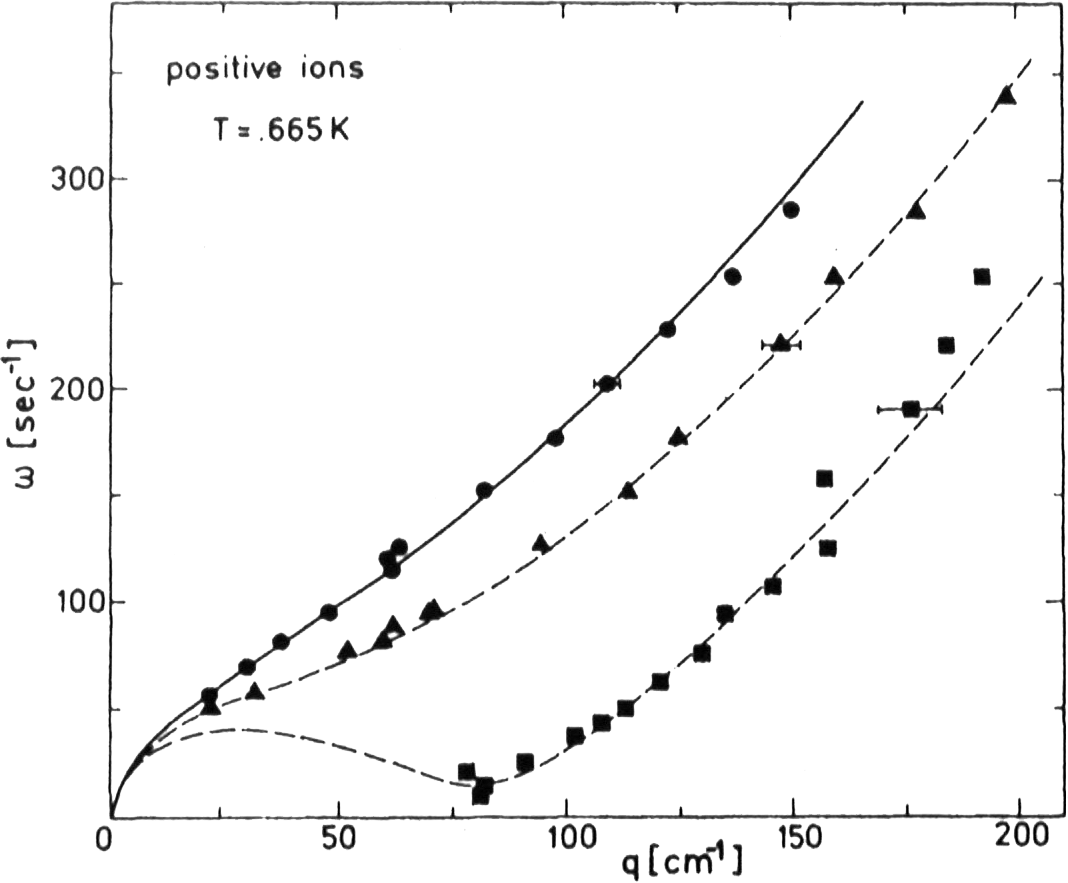
\includegraphics[width=\smallwidth]{theo_electrons_on_helium/instability}\hfill
    \begin{minipage}[b]{\textwidth-\smallwidth-2\tabcolsep}
        \caption[Ripplonendispersionsrelation an der Grenzfläche einer gesättigten $^3$He"=$^4$He"=Mischung]{Ripplonendispersionsrelation an der Grenzfläche einer gesättigten $^3$He"=$^4$He"=Mischung nach \name{Leiderer} \cite{Lei79}. Die Grenzfläche ist von unten mit positiven Ionen beladen.\par$T=\unit[0.665]{K}$, $n_c=\unit[4.8\times10^{12}]{\Em}$, $E_c=\unitfrac[87.5]{kV}{m}$. $E/E_c=0.12$ ({\large$\bullet$}), 0.71 ($\blacktriangle$) und 0.995 ({\tiny$\blacksquare$}).}
        \label{fig:bulk_instability}
    \end{minipage}
\end{figure}

Für ungesättigte Elektronendichten, $n<n_{s,\text{crit}}$, d.~h.\ für geringere Elektronendichten aber höhere Haltespannungen, kann ebenfalls ein so hoher Elektronendruck erreicht werden, der auch in diesem Fall zu einer Instabilität und somit zum Einbrechen von Elektronen in das Bulk"=Helium führen kann.

Das Auftreten der elektrohydrodynamischen Instabilität kann bei Messungen von 2DES auf Bulk"=Helium auch als Eichpunkt für die Elektronendichte herangezogen werden. Dies wird später z.\ B.\ bei der Bestimmung der Elektronenproduktion der Filamente in Abschnitt~\ref{ssec:electron_production} und zur Eichung des Kondensators zur Bestimmung der Helium"=Füllhöhe in \ref{ssec:level_calib} Verwendung finden.

\begin{figure}[h!tbp]
    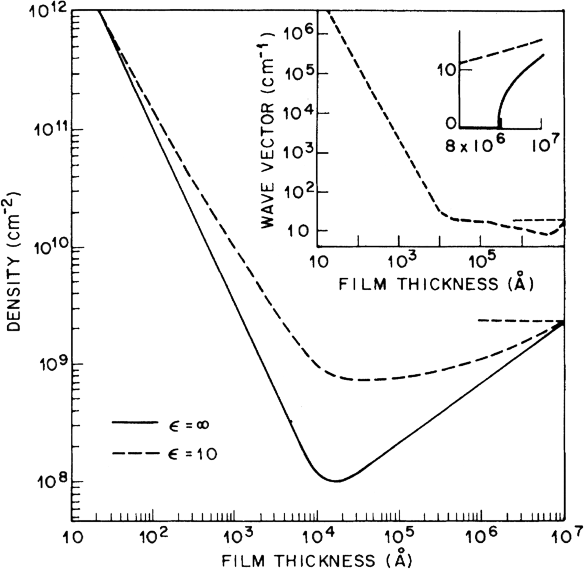
\includegraphics[width=\smallwidth]{theo_electrons_on_helium/stability}\hfill
    \begin{minipage}[b]{\textwidth-\smallwidth-2\tabcolsep}
        \caption[Kritische Elektronendichten der elektrohydrodynamischen Instabilität.]{Abhängigkeit der kritischen Elektronendichte der elektrohydrodynamischen Instabilität nach \name{F. Peeters} \cite{Pee84} von der Dicke der Heliumschicht zwischen Substrat und 2DES für ein metallisches (durchgezogene Linie) und ein nicht"=metallisches Substrat. Im Einsatz ist die Wellenzahl aufgetragen, an der die Instabilität zuerst auftritt (vgl.\ hierzu Abb.~\ref{fig:bulk_instability}).}
        \label{fig:bulk_instability_dep}
    \end{minipage}
\end{figure}

Um die Beschränkung der maximal erreichbaren Elektronendichte zu umgehen, kann man, wie bereits in \cite{Ike81}, \cite{Mon82} und \cite{Wil82} vorgeschlagen, zu gesättigten Heliumfilmen als Unterlage für die Elektronen übergehen. Hier wird die Ripplonendispersionsrelation \eqref{eqn:ripplon_dispersion:film} durch die starke van"=der"=Waals"=Wechselwirkung zwischen den Heliumatomen und dem darunter liegendem Substrat derart modifiziert, dass die Erhöhung der Elektronendichte nicht zu einer Instabilität führt. Dies wird später in Abschnitt~\ref{ssec:film_stability} genauer untersucht.

\subsection{Die Beweglichkeit der Elektronen im 2DES}
\label{ssec:mobility}
Ohne äußeres elektrisches Feld ist die Geschwindigkeit der Elektronen $\vec v$ im Mittel gleich Null. Bei Anwesenheit eines elektrischen Feldes werden die Elektronen beschleunigt. Stellt man sich ein Elektron zur Zeit $t=0$ vor, dann ist $t$ die Zeit, die seit der letzten Kollision vergangen ist. Ein äußeres Feld ändert die Geschwindigkeit um $-e\vec E\frac{t}{m}$, was sich aus
    \begin{equation}
        F=m_ea\quad\Rightarrow\quad a=\frac{F}{m_e}\quad\Rightarrow\quad v=at=\frac{Ft}{m_e}
    \end{equation}
ergibt. Die durchschnittliche Geschwindigkeit $\vec v_\text{avg}$ und die Beweglichkeit $\mu$ der Elektronen wird bestimmt durch die mittlere Streuzeit $\tau$:
    \begin{equation}
        \vec v_\text{avg}=-\frac{e\vec E\tau}{m_e}\ttextt{und}		\mu=\frac{e\,\tau}{m_e}\quad.
    \end{equation}

Eingesetzt in die Gleichung für die Stromdichte $j=n e \vec v$ ergibt sich das Drude"=Gesetz für die Gleichstromleitung in einem metallischen Leiter:
	$\vec j = \sigma\vec E$ mit der Leitfähigkeit $\sigma$: $\sigma=n e \mu$.

\subsection{Elektronen im elektrischen Wechselfeld}
\label{ssec:eqns_of_motion}
Aus der klassischen Bewegungsgleichung eines einzelnen Elektrons im elektrischen Feld $\vec E$ mit einem Lokalisierungspotential der Frequenz $\omega_0$ und einer mittleren Stoßzeit $\tau$, 
\begin{equation}
		m\ddot{\vec x}+\frac{m}{\tau}\dot{\vec x}+m\omega_0^2\vec x=e\vec E
\end{equation}
kann man über einen harmonischen Lösungsansatz $\vec x, \vec E\propto e^{i\omega t}$ aus dem Realteil der Lösung für die Geschwindigkeit $\vec v$ des Elektrons, die Dissipation $P$ des Elektronensystems bestimmen:
\begin{equation}
	P=\frac{m}{\tau}\vec v\vec v^*=\frac{Ne^2}{m}\tau\frac{1}{1+\left(\frac{\omega_0^2-\omega^2}{\omega}\right)^2\tau^2}E^2\quad.
\end{equation}

Aus dem Realteil der Ortsfunktion $\vec x$ läßt sich über das Gesamtdipolmoment der Elektronen $\vec P=N\vec p=N\,e\,\vec x$ analog die Suszeptibilität des Elektronensystems bestimmen:
\begin{equation}
\chi=\frac{\left|\vec P\right|}{\varepsilon_0E}=\frac{Ne^2}{m}\tau^2\frac{(\omega_0^2-\omega^2)\tau^2}{\left(\omega_0^2-\omega^2\right)^2\tau^4+\omega^2\tau^2}\quad.
\end{equation}

\subsection{Wichtige Streumechanismen}
\label{ssec:scattering}

\begin{figure}[h!tp]
	\hfill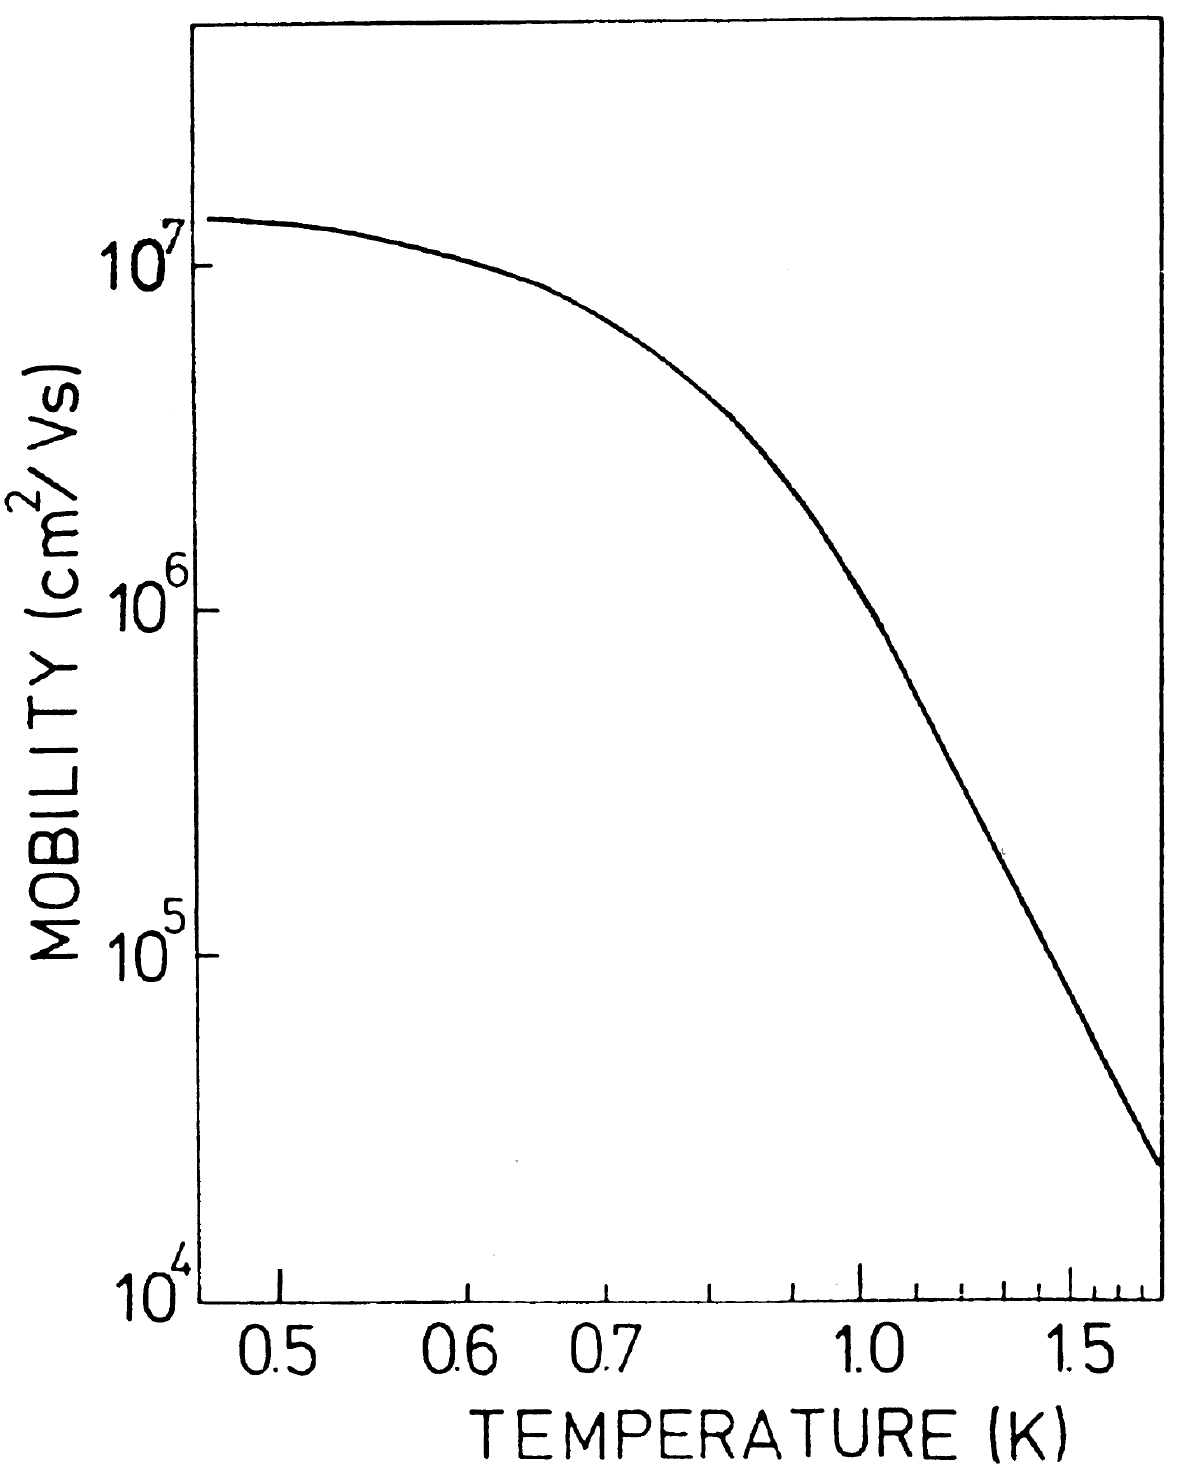
\includegraphics[width=2in]{theo_electrons_on_helium/mobility}\hfill
	\begin{minipage}[b]{\textwidth-\smallwidth-2\tabcolsep}
		\caption[Temperaturabhängigkeit der Beweglichkeit von Elektronen auf Bulk"=Helium]{Messung der Beweglichkeit von Elektronen auf Bulk"=Helium aus \cite{Lei92}. Deutlich sieht man die im Text beschriebene exponentielle Temperaturabhängigkeit im Regime der Gasatomstreuung oberhalb von ca.\ \unit[0.8]{K} und die schwache Temperaturabhängigkeit im Regime der Streuung an Ripplonen unterhalb von ca.\ \unit[0.7]{K}.\label{fig:mobility}}
	\end{minipage}
\end{figure}

Die Elektronen über der Oberfläche von flüssigem Helium werden auf Grund von verschiedenen Mechanismen gestreut. Oberhalb von ca.\ \unit[0.8]{K} dominiert die Streuung an den Helium"=Gasatomen, die mit der Temperatur exponentiell zunimmt. Dies wurde von \name{Sommer} \ea \cite{Som71} experimentell nachgewiesen. Unterhalb von \unit[0.7]{K} ist nur noch die Streuung an den Ripplonen der Heliumoberfläche dominierend -- experimenteller Nachweis durch \name{Grimes} \ea \cite{Gri76} -- die allerdings auf Grund der schwachen Temperaturabhängigkeit der Anregung von Ripplonen die Beweglichkeit der Elektronen kaum beeinflusst (siehe auch \cite{Bri77,Col74}). Auf dünnen Heliumfilmen bestehen auf Grund der Rauigkeit des Substrats viele Streuzentren, die dann die Beweglichkeit der Elektronen um einige Größenordnungen reduzieren. 
